%% !TEX program = lualatex
%% !TEX TS-program = lualatex
% !TEX encoding = UTF-8 Unicode
% !TEX spellcheck = en_GB
\documentclass{beamer}

% \graphicspath{{./graphics/}}

% ====================
% Packages
% ====================

\usepackage[T1]{fontenc}
\usepackage{lmodern}
% \usepackage[size=a4,scale=1.1]{beamerposter}
\usepackage[size=a1,scale=1.0]{beamerposter}
% \usepackage[size=custom,height=100,width=70.71,scale=1.2]{beamerposter}
% \usepackage[size=a4,scale=1.0,orientation=landscape]{beamerposter}

\usetheme{gemini}
\usecolortheme{poster}
\usefonttheme{default}

\usepackage{graphicx}
\usepackage{booktabs}
\usepackage{tikz}
\usepackage{pgfplots}
\pgfplotsset{compat=1.17}
\usepackage{multicol}
% \usepackage{enumerate}
% \usepackage{enumitem}
\usepackage{caption}
\captionsetup{font=normalsize}
% ====================
% Lengths
% ====================

% If you have N columns, choose \sepwidth and \colwidth such that
% (N+1)*\sepwidth + N*\colwidth = \paperwidth
% \colwidth = 1pt * \ratio{\paperwidth - {\ncols+1}\sepwidth}{\ncols}
\newcommand{\ncols}{3}
\newlength{\sepwidth}
\newlength{\colwidth}
\newlength{\midspace}
\setlength{\sepwidth}{0.020\paperwidth}
% \setlength{\colwidth}{0.32\paperwidth}
\setlength{\colwidth}{
{\dimexpr \paperwidth / \ncols \relax} -
{\dimexpr \sepwidth + \sepwidth / \ncols \relax}
}
\setlength{\midspace}{20ex}

\newcommand{\separatorcolumn}{\begin{column}{\sepwidth}\end{column}}

% ====================
% Title
% ====================

\title{Software Interface Design for a Full-Duplex Embedded System}

\author{\textbf{Student:} Taharka Okai}

\institute[shortinst]{University of Bristol, Dept. of Engineering}

\newcommand{\beamerblocknoheader}{
  \setbeamertemplate{block begin}{
    {\parskip0pt\par}
    \usebeamerfont{block body}
    \vskip-0.5ex
    \begin{beamercolorbox}[colsep*=0ex]{block body}
    \justifying
    \setlength{\parskip}{1ex}
    \vskip-2ex
  }

  \setbeamertemplate{block alerted begin}{
    % \begin{beamercolorbox}[colsep*=0ex,dp=2ex,center]{block alerted title}
    %   \vskip0pt
    %   \usebeamerfont{block title}\insertblocktitle
    %   \vskip-1.25ex
    %   \begin{beamercolorbox}[colsep=0.025ex]{block alerted separator}\end{beamercolorbox}
    % \end{beamercolorbox}
    {\parskip0pt\par}
    \usebeamerfont{block body}
    \vskip-0.5ex
    \begin{beamercolorbox}[colsep*=0ex]{block alerted body}
    \justifying
    \begin{adjustwidth}{1ex}{1ex}
    \setlength{\parskip}{1ex}
    \vskip-2ex
  }
}

\newcommand{\beamerblockheader}{
\setbeamertemplate{block begin}{
\begin{beamercolorbox}[colsep*=0ex,dp=2ex,center]{block title}
  \vskip0pt
  \usebeamerfont{block title}\insertblocktitle
  \vskip-1.25ex
  \begin{beamercolorbox}[colsep=0.025ex]{block separator}\end{beamercolorbox}
\end{beamercolorbox}
{\parskip0pt\par}
\usebeamerfont{block body}
\vskip-0.5ex
\begin{beamercolorbox}[colsep*=0ex]{block body}
\justifying
\setlength{\parskip}{1ex}
\vskip-2ex
}

\setbeamertemplate{block alerted begin}{
\begin{beamercolorbox}[colsep*=0ex,dp=2ex,center]{block alerted title}
  \vskip0pt
  \usebeamerfont{block title}\insertblocktitle
  \vskip-1.25ex
  \begin{beamercolorbox}[colsep=0.025ex]{block alerted separator}\end{beamercolorbox}
\end{beamercolorbox}
{\parskip0pt\par}
\usebeamerfont{block body}
\vskip-0.5ex
\begin{beamercolorbox}[colsep*=0ex]{block alerted body}
\justifying
\begin{adjustwidth}{1ex}{1ex}
\setlength{\parskip}{1ex}
\vskip-2ex
}
}


% ====================
% Footer (optional)
% ====================

\footercontent{
  % \href{https://www.example.com}{https://www.example.com} \hfill
  % ABC Conference 2025, New York --- XYZ-1234 \hfill
  % \href{mailto:a.kalay@example.com}{a.k@example.com}
}


\abovefooter{
  % \hfill\includegraphics[height=9ex]{uoblogo.png}
}
% (can be left out to remove footer)

% ====================
% Logo (optional)
% ====================

% use this to include logos on the left and/or right side of the header:
% \logoright{\includegraphics[height=2cm]{uoblogo.png}}
% \logoleft{\includegraphics[height=5pt]{graphics/uoblogo.png}}

\hypersetup{
  pdfauthor={Taharka Okai},
  pdftitle={Designing a Sketch Based Interface for Electronic Circuit Simulation},
  pdfsubject={Poster},
  pdfkeywords={Electronic Circuit Simulation, Sketch Recognition, Computer Vision, Machine Learning},
  pdfstartview={FitH},
  pdfpagemode={UseOutlines},
  pdfpagelayout={SinglePage},
  pdfborder={0 0 0},
}


\date{\today}

\begin{document}

\begin{frame}[t]
  \begin{columns}[t]

    \separatorcolumn

    \begin{column}{\colwidth}
      \begin{block}{1. Project Background}
        Circuit simulation is a well-known and useful computer-aided design
        (CAD) tool for designing electronic circuits. However, ease of use and
        speed of prototyping are two major drawbacks of circuit simulation using
        traditional CAD tools.

        Additionally, there is an increasing trend in the use of machine learning
        tools to aid research and development \cite{review/Moreno-Garcia2019}.
        Using recent advances in computer vision research and machine learning to
        develop a tool that can quickly and accurately interpret hand-drawn diagrams.
      \end{block}


      \begin{block}{2. Project Outcome}
        This project aims to produce a software tool that receives hand-drawn
        circuit diagrams as input and generates an LT-SPICE simulation file as output,
        which will be paired with a compatible backend to produce a fully functional
        circuit simulation tool. The user will be able to:

        \begin{itemize}
          \item Draw a circuit diagram on paper/whiteboard/tablet/digital image
          \item Pass the sketch to the application
          \item Simulate/download the simulation file on their device
        \end{itemize}
      \end{block}


      \begin{block}{3. Existing Solutions}
        There are a number of existing solutions that are similar to the project
        outcome. These methods each have their own merits and drawbacks, as detailed
        below:

        \begin{itemize}
          \item \textbf{Programmatic}:
                \cite{}: use image processing and properties of the shapes of
                the circuit components to identify them.
          \item \textbf{Support Vector Machines}:
                \cite{}: use a Support Vector Machine (SVM) to classify the components
                of the circuit.
          \item \textbf{Object Detection}: \cite{dl/Rachala2022,dl/Dey2021}: use deep learning to classify
                the components of the circuit.
        \end{itemize}

        These approaches \cite{} require intimate knowledge of the geometry of the components
        and the image processing techniques required to extract the relevant information
        from the image.

        Additionally, only a few of these solutions \cite{} go on to produce the file required
        for simulation, and less still \cite{} produce a fully functional simulation tool.
      \end{block}

      {\beamerblocknoheader
      \vspace*{2ex}
      \begin{block}{}
        \begin{figure}[t]
          \centering
          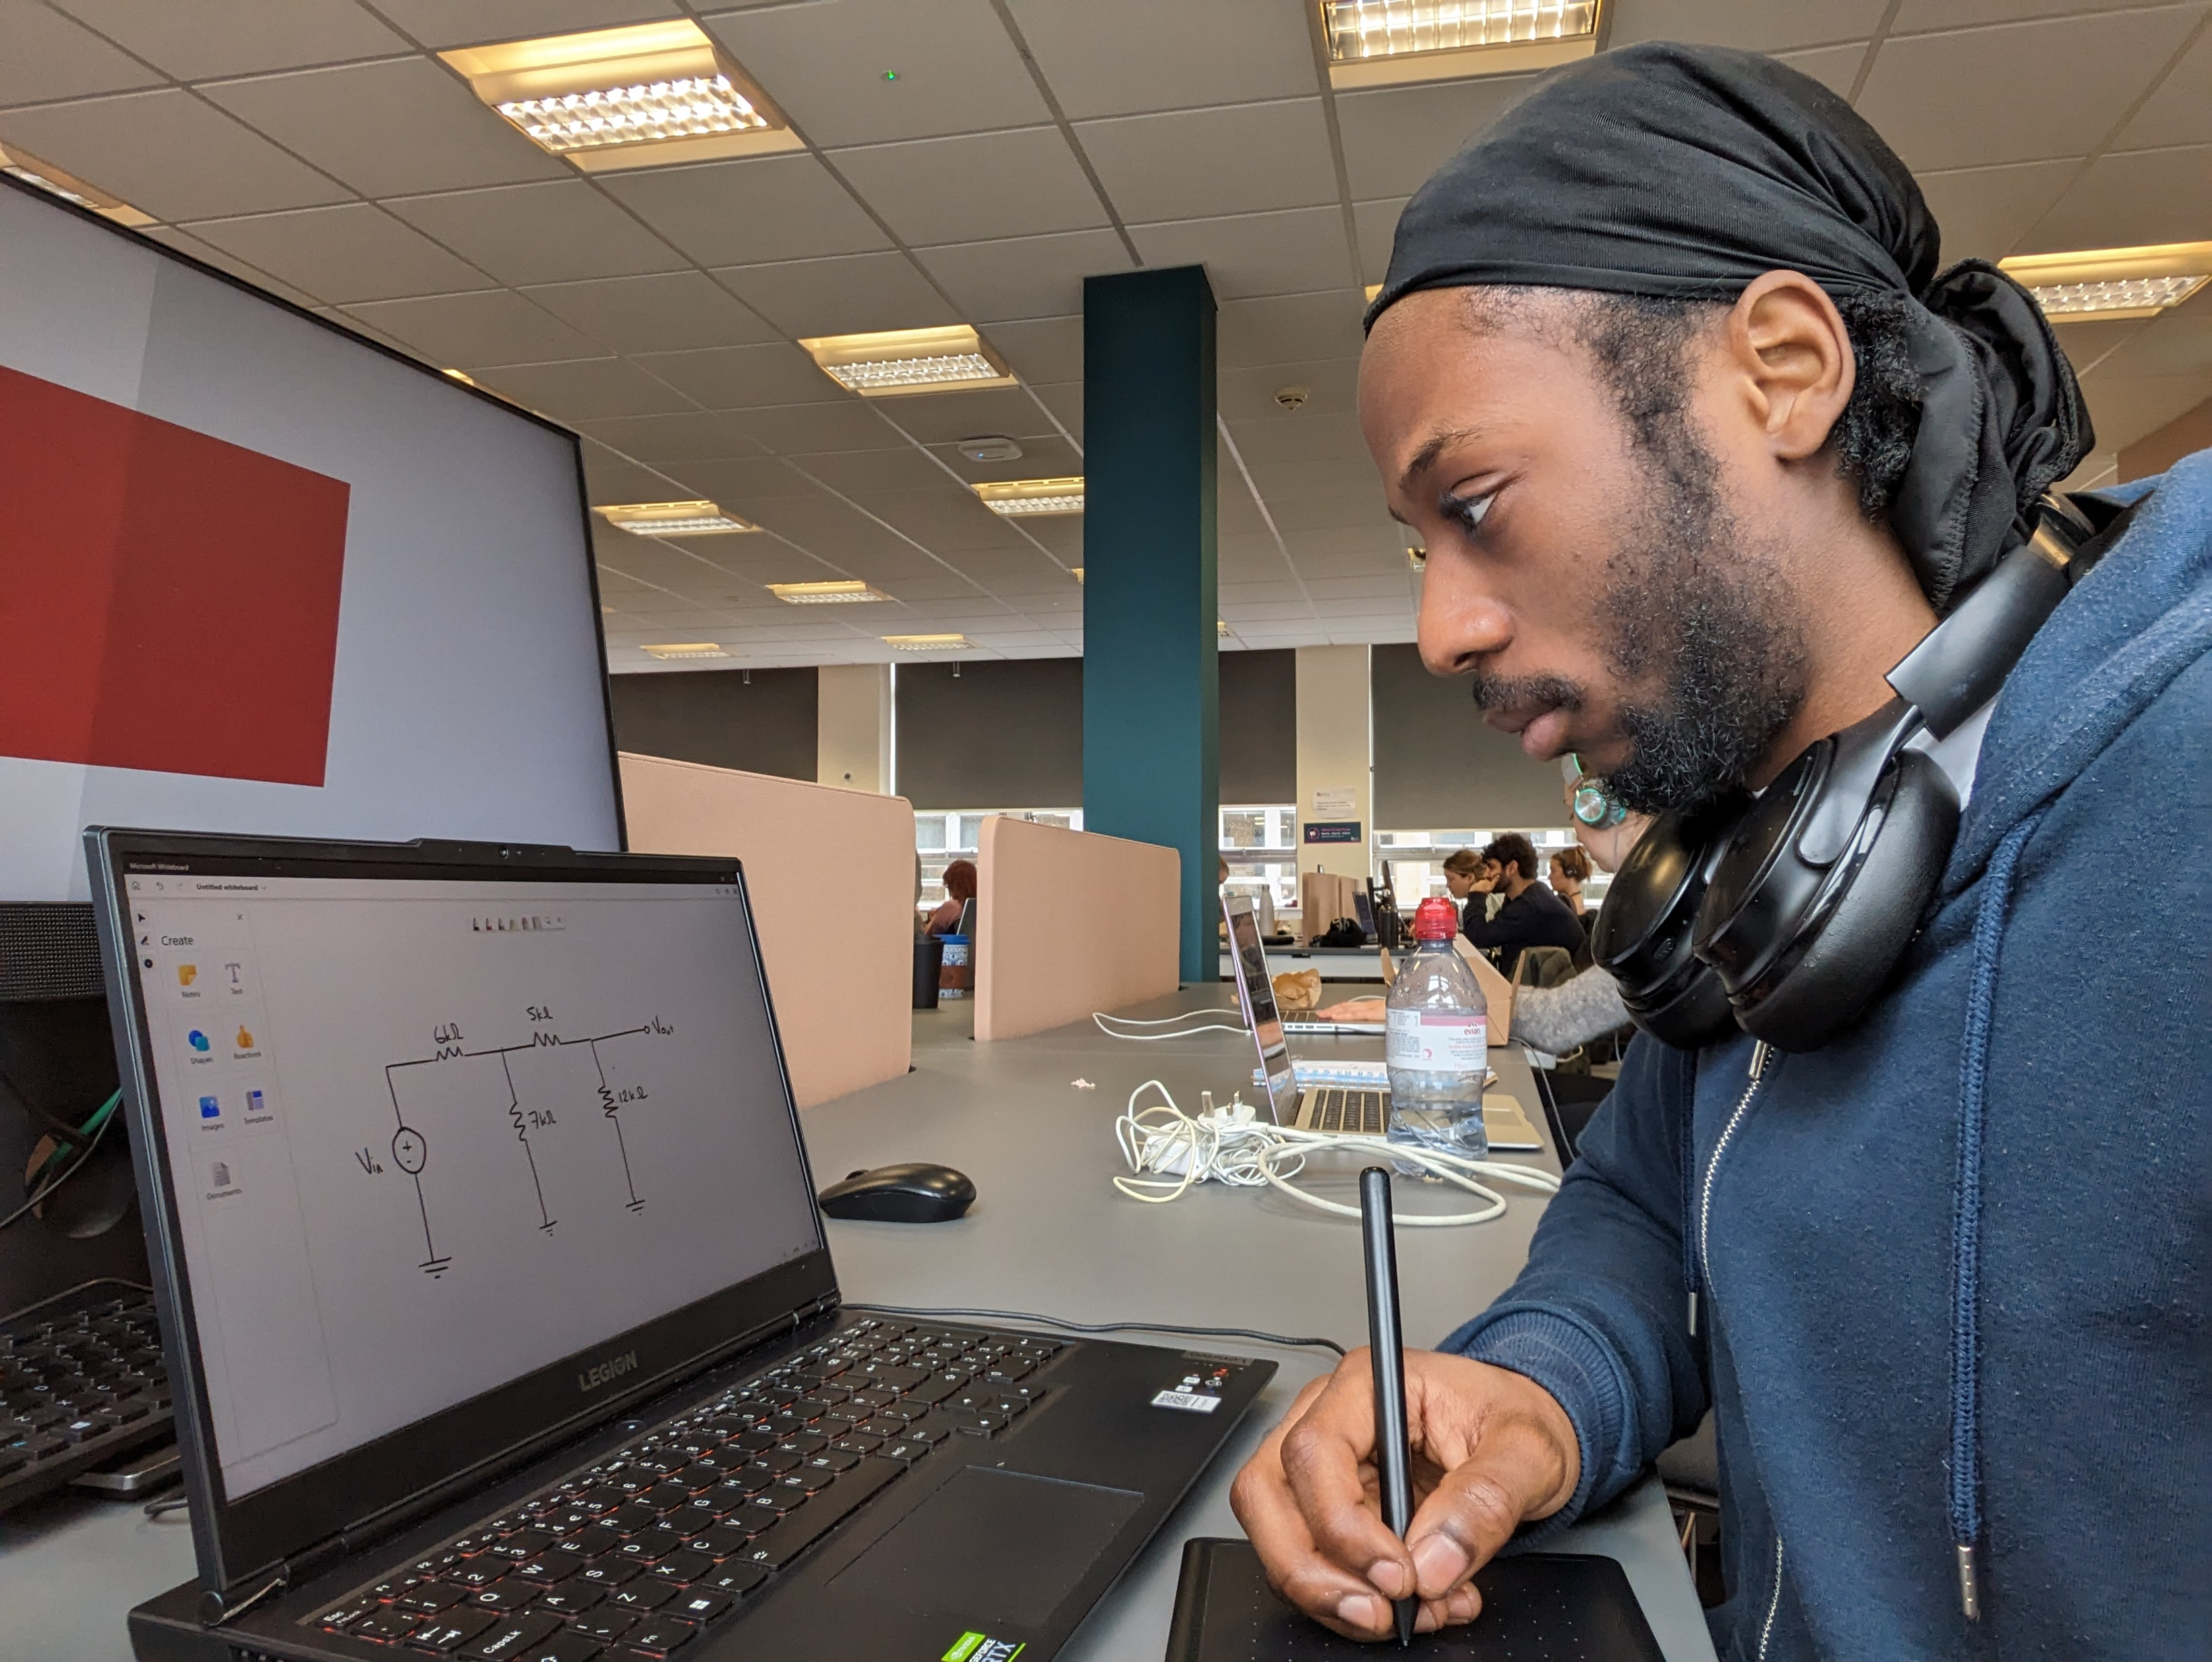
\includegraphics[keepaspectratio,width=\colwidth,height=40ex]{../common/graphics/demonstration-draw.jpg}
          % \resizebox{\colwidth}{!}{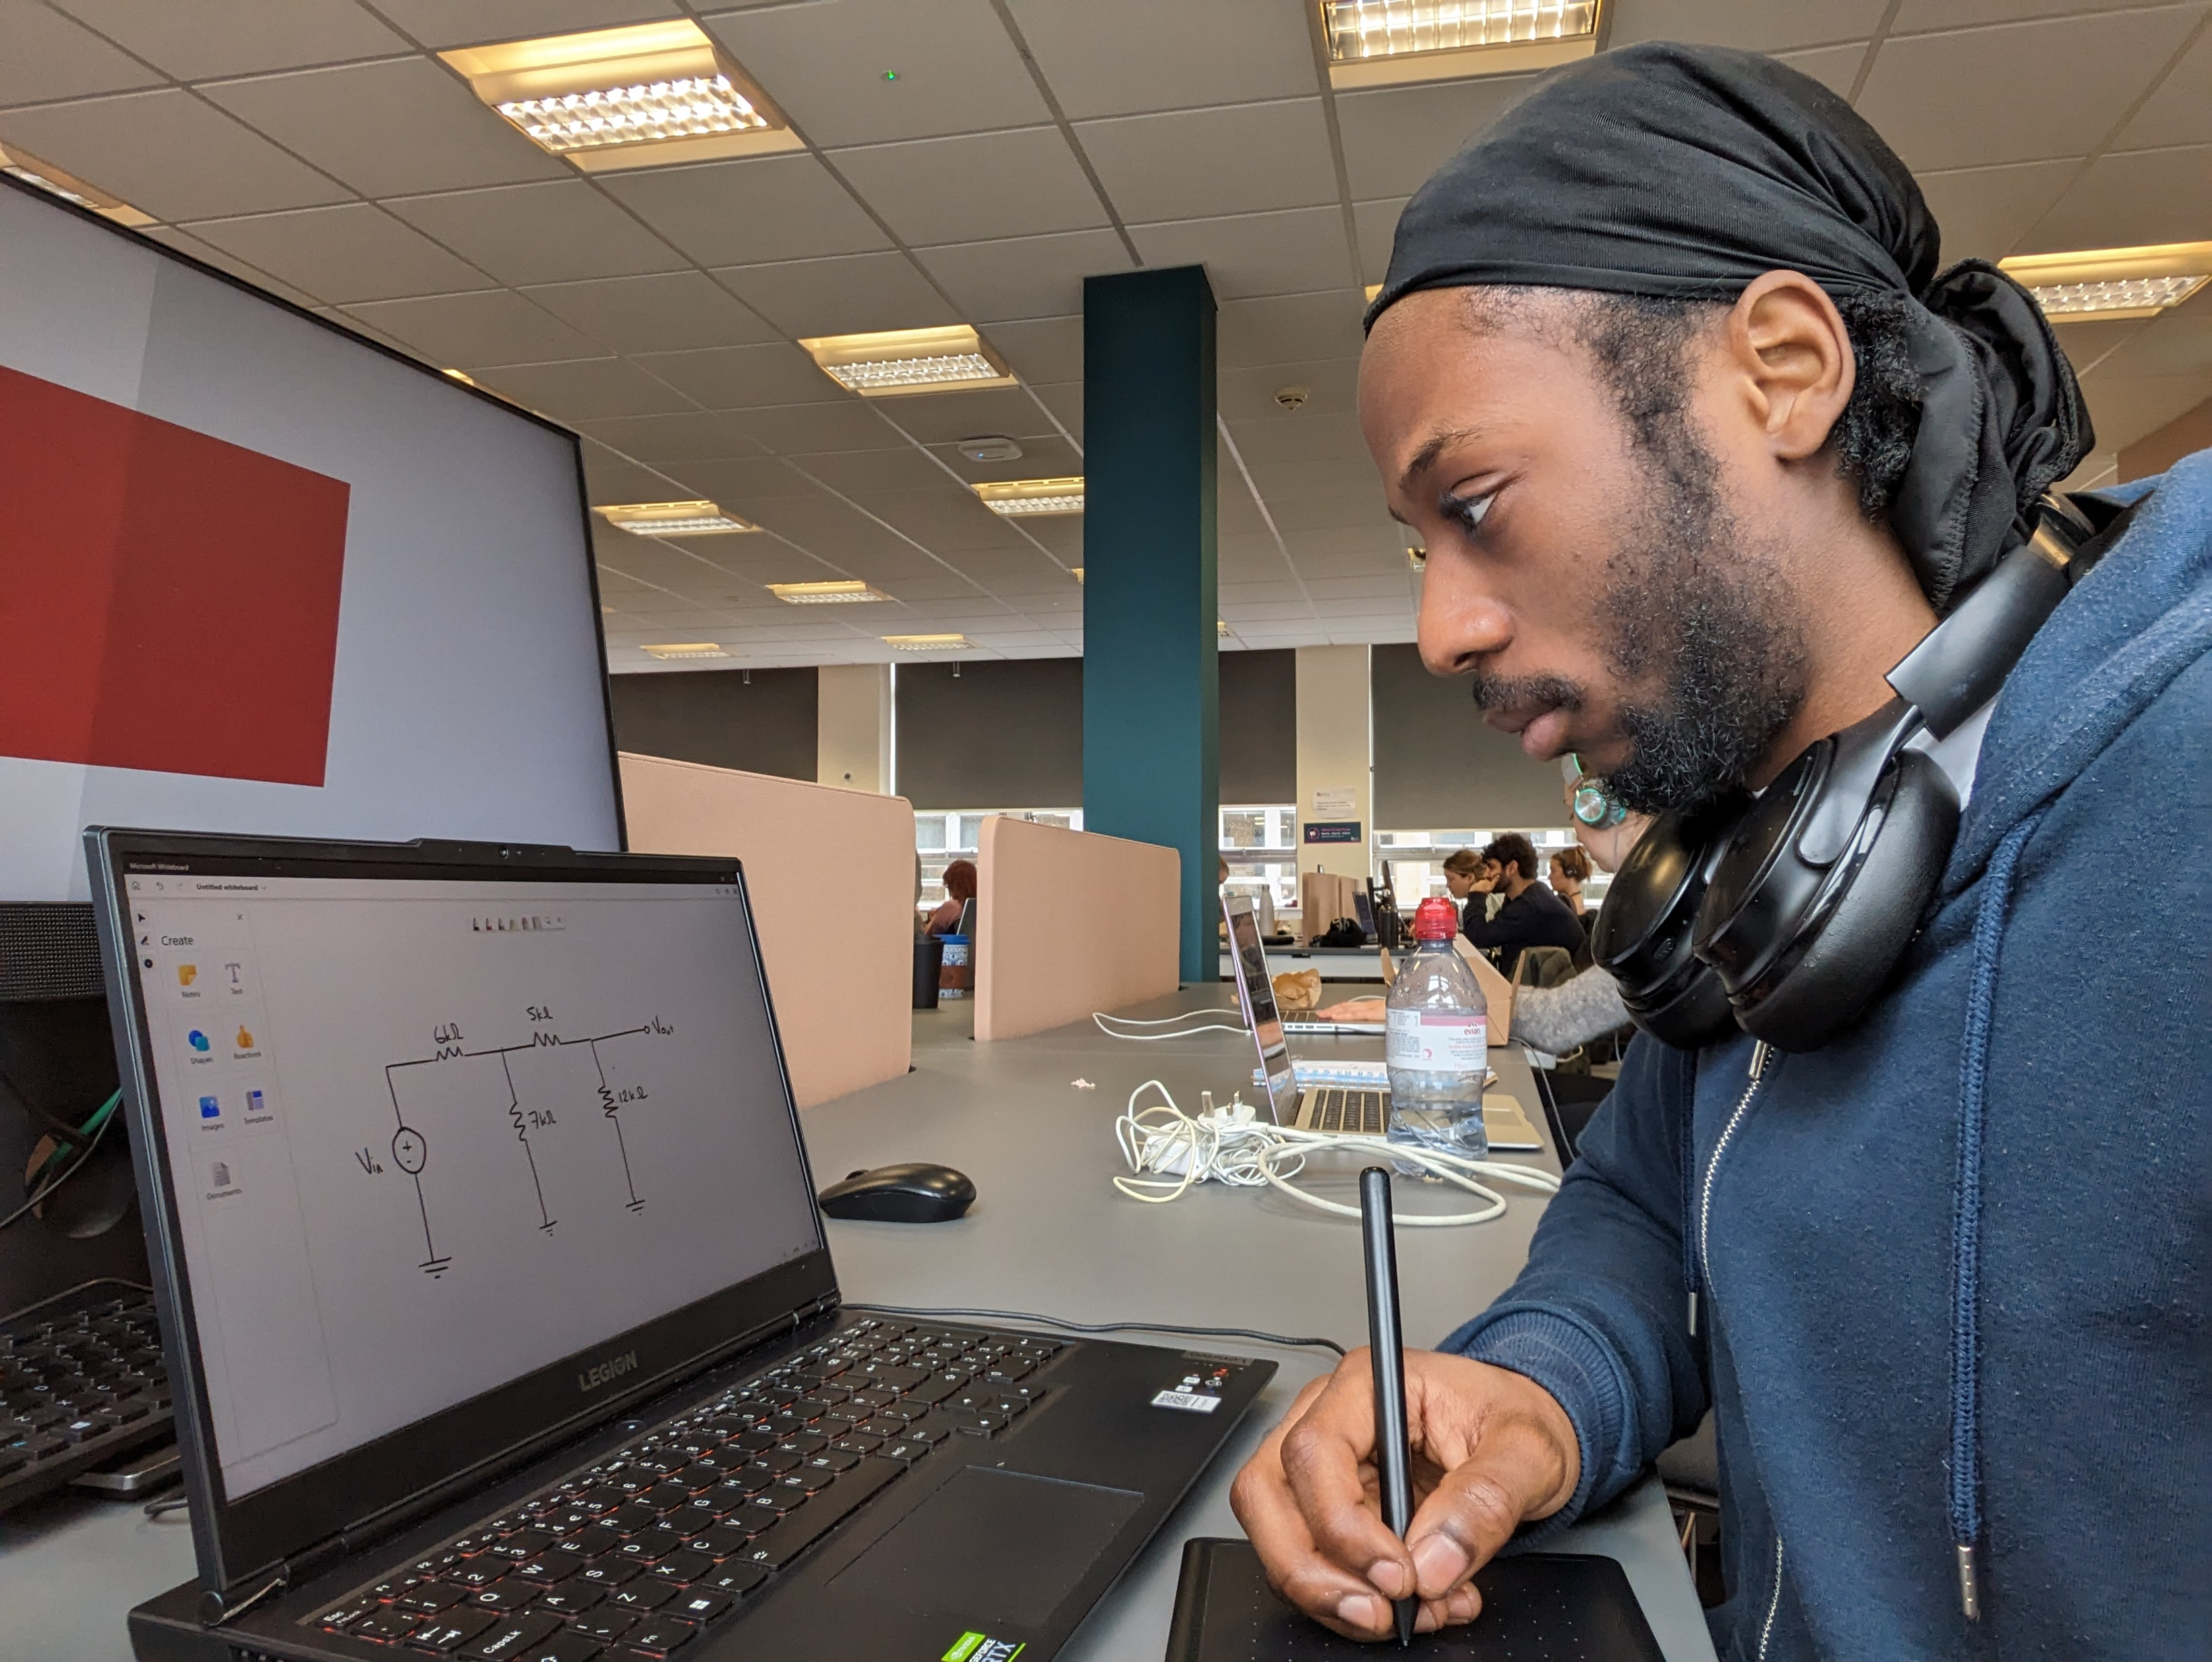
\includegraphics{../common/graphics/demonstration-draw.jpg}}
          \caption{Creating a digital image of the circuit diagram}
          \label{key1}
        \end{figure}
      \end{block}
      }

    \end{column}

    \separatorcolumn

    \begin{column}{\colwidth}
      {\beamerblocknoheader
        \begin{block}{}
          \centering
          \begin{figure}[t]
            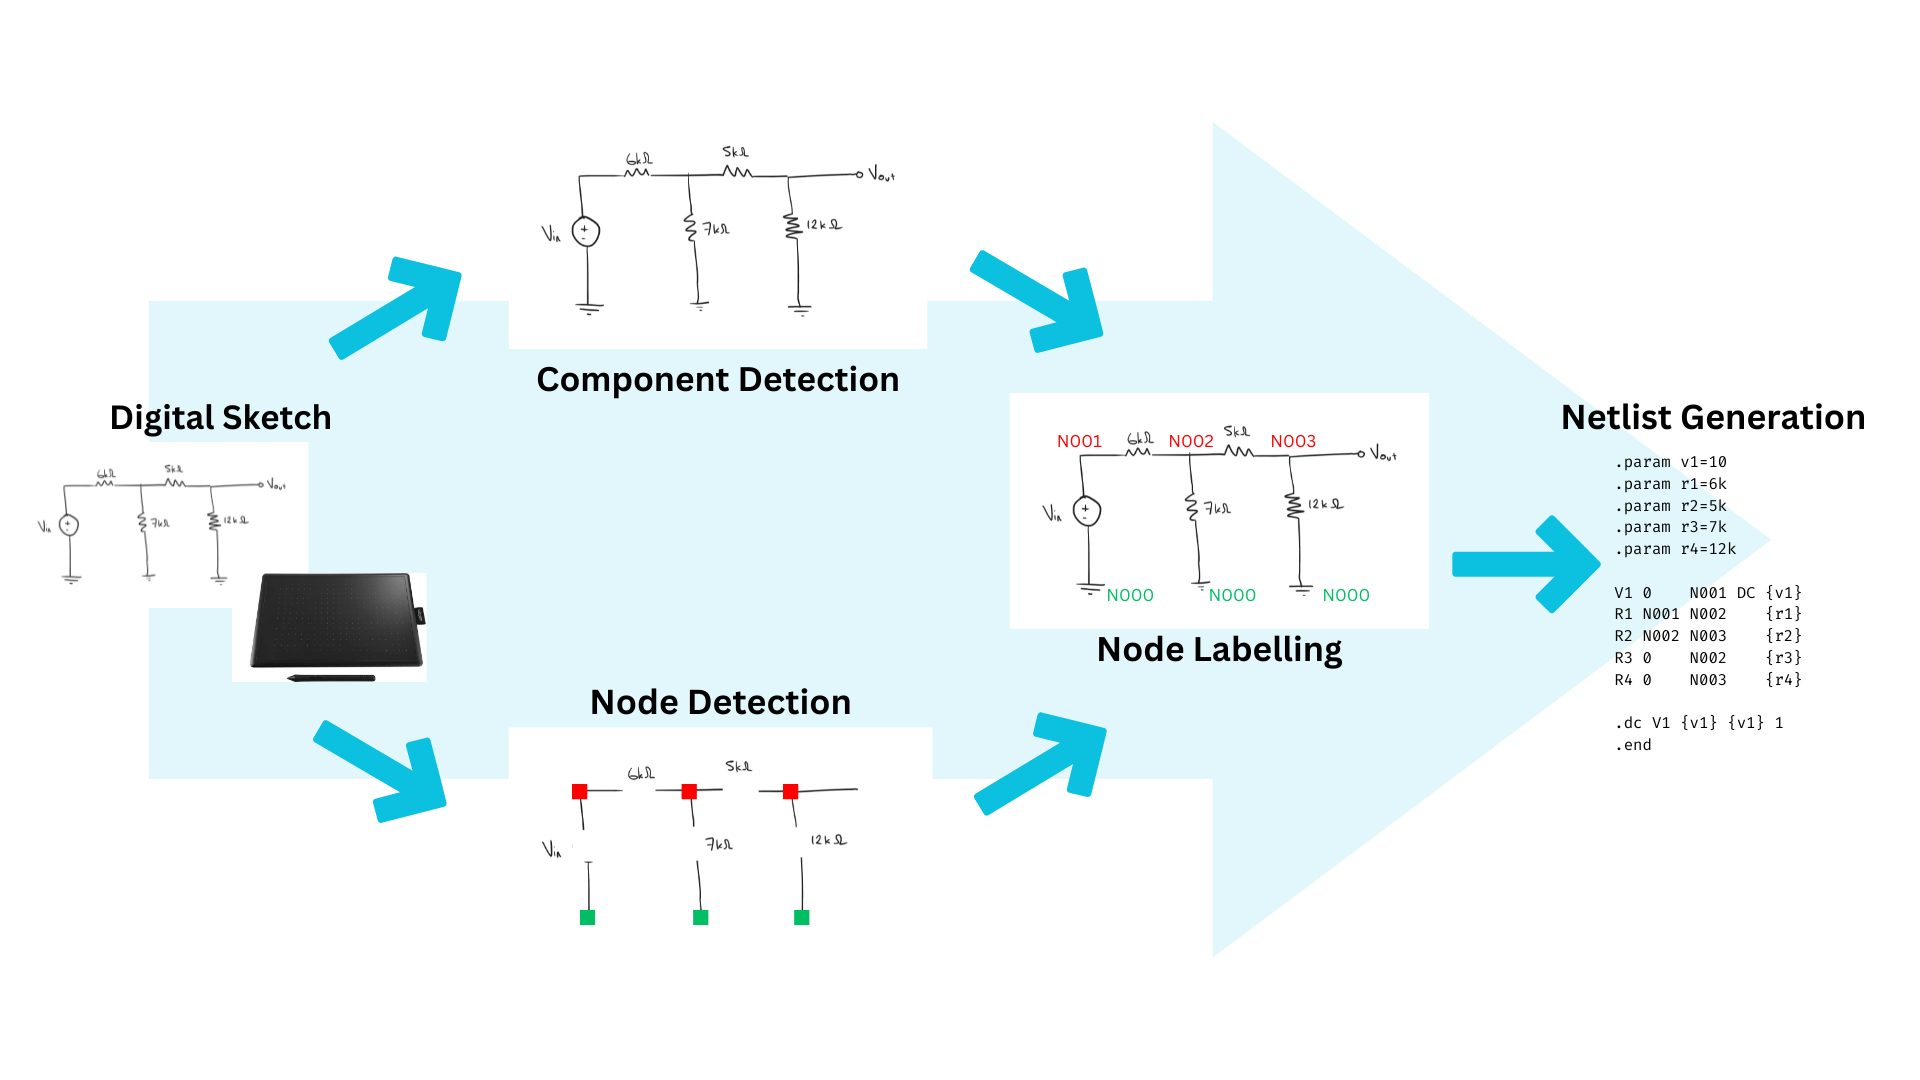
\includegraphics[width=\colwidth,height=40ex]{../common/graphics/create-representation}
            \caption{Creating a representation of the circuit diagram in software}
            \label{ke2}
          \end{figure}
        \end{block}
      }
      {\beamerblocknoheader
        % \beamerboxesrounded
        \begin{alertblock}{}
          \centering
          \begin{column}{\colwidth-\sepwidth}
            {\beamerblockheader
              \setbeamercolor{block body}{bg=,fg=white}
              \setbeamercolor{block title}{bg=,fg=white}
              \setbeamercolor{block separator}{bg=white}
              \setbeamertemplate{itemize item}{\raise0.5ex \hbox{{\color{white}\vrule width 0.5ex height 0.5ex}}}
              \setbeamertemplate{itemize subitem}{\raise0.3ex \hbox{{\color{white}\vrule width 0.5ex height 0.5ex}}}
              \RaggedRight

              \begin{block}{4. Methodology}
                \RaggedRight
                Firstly, a model was trained to create a representation of the circuit:
                \begin{itemize}
                  \item \textbf{Data collection} -- labelled images of circuit diagrams
                  \item \textbf{Preprocessing} -- Contrast Limited Adaptive Histogram Equalisation (CLAHE)
                  \item \textbf{Training and Validation} -- 80/10/10 train/test/validation split
                \end{itemize}

                \RaggedRight
                Then, the hand-drawn circuits go through the following steps to produce a simulation file:
                \begin{itemize}
                  \RaggedRight
                  \item \textbf{Component/Node Detection} -- YOLOv8 bounding box and Hough Transform used to detect components and nodes
                  \item \textbf{Node Labelling} -- Graph representation of the circuit is generated
                  \item \textbf{Simulation} The simulation file is passed to a Python wrapper around LT-SPICE
                        to produce a simulation
                \end{itemize}
              \end{block}
            }
          \end{column}
        \end{alertblock}
      }
      {\beamerblocknoheader
        \begin{block}{}
          \begin{figure}[t]
            \centering
            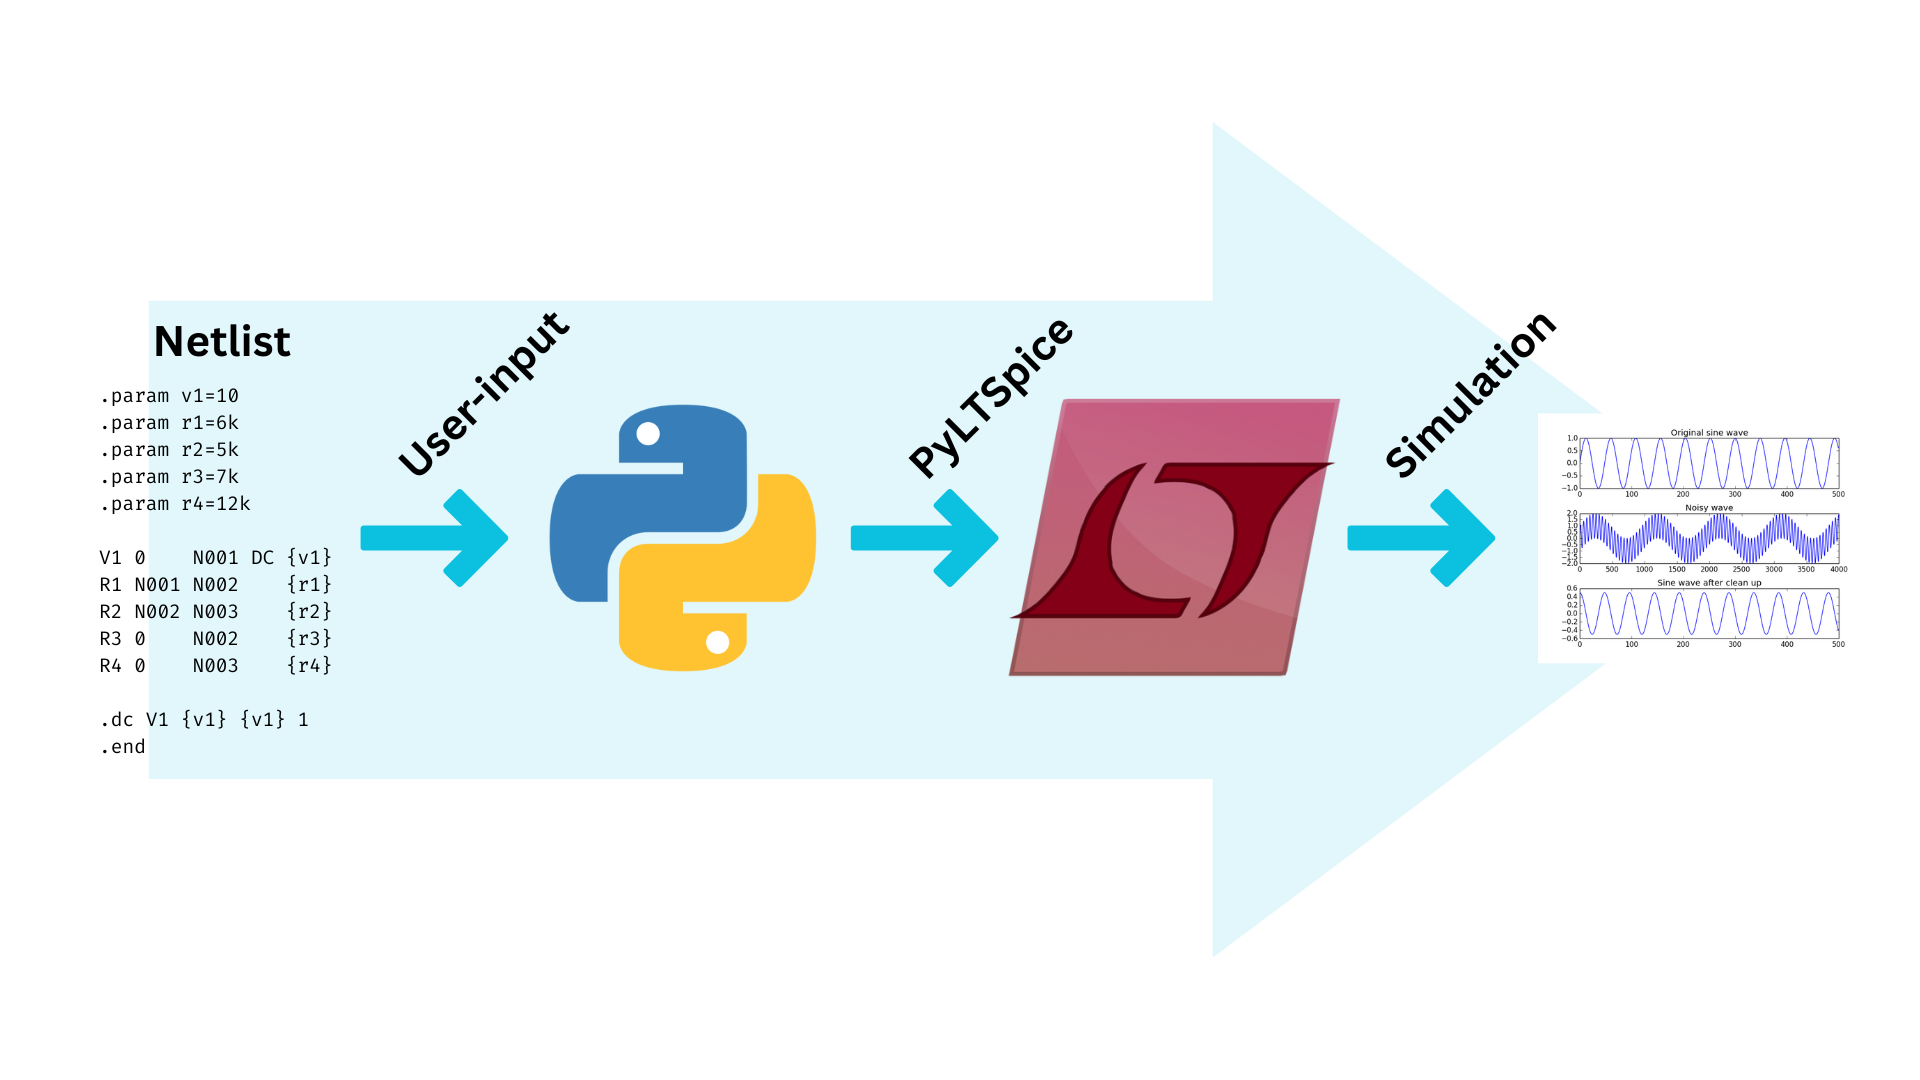
\includegraphics[width=\colwidth,height=40ex]{../common/graphics/create-simulation}
            \caption{Simulating the digital representation of the circuit diagram}
            \label{key3}
          \end{figure}
        \end{block}
      }
    \end{column}

    \separatorcolumn

    \begin{column}{\colwidth}

      {\beamerblocknoheader
        \begin{block}{}
          \begin{figure}[t]
            \centering
            \begin{subfigure}{0.45\textwidth}
              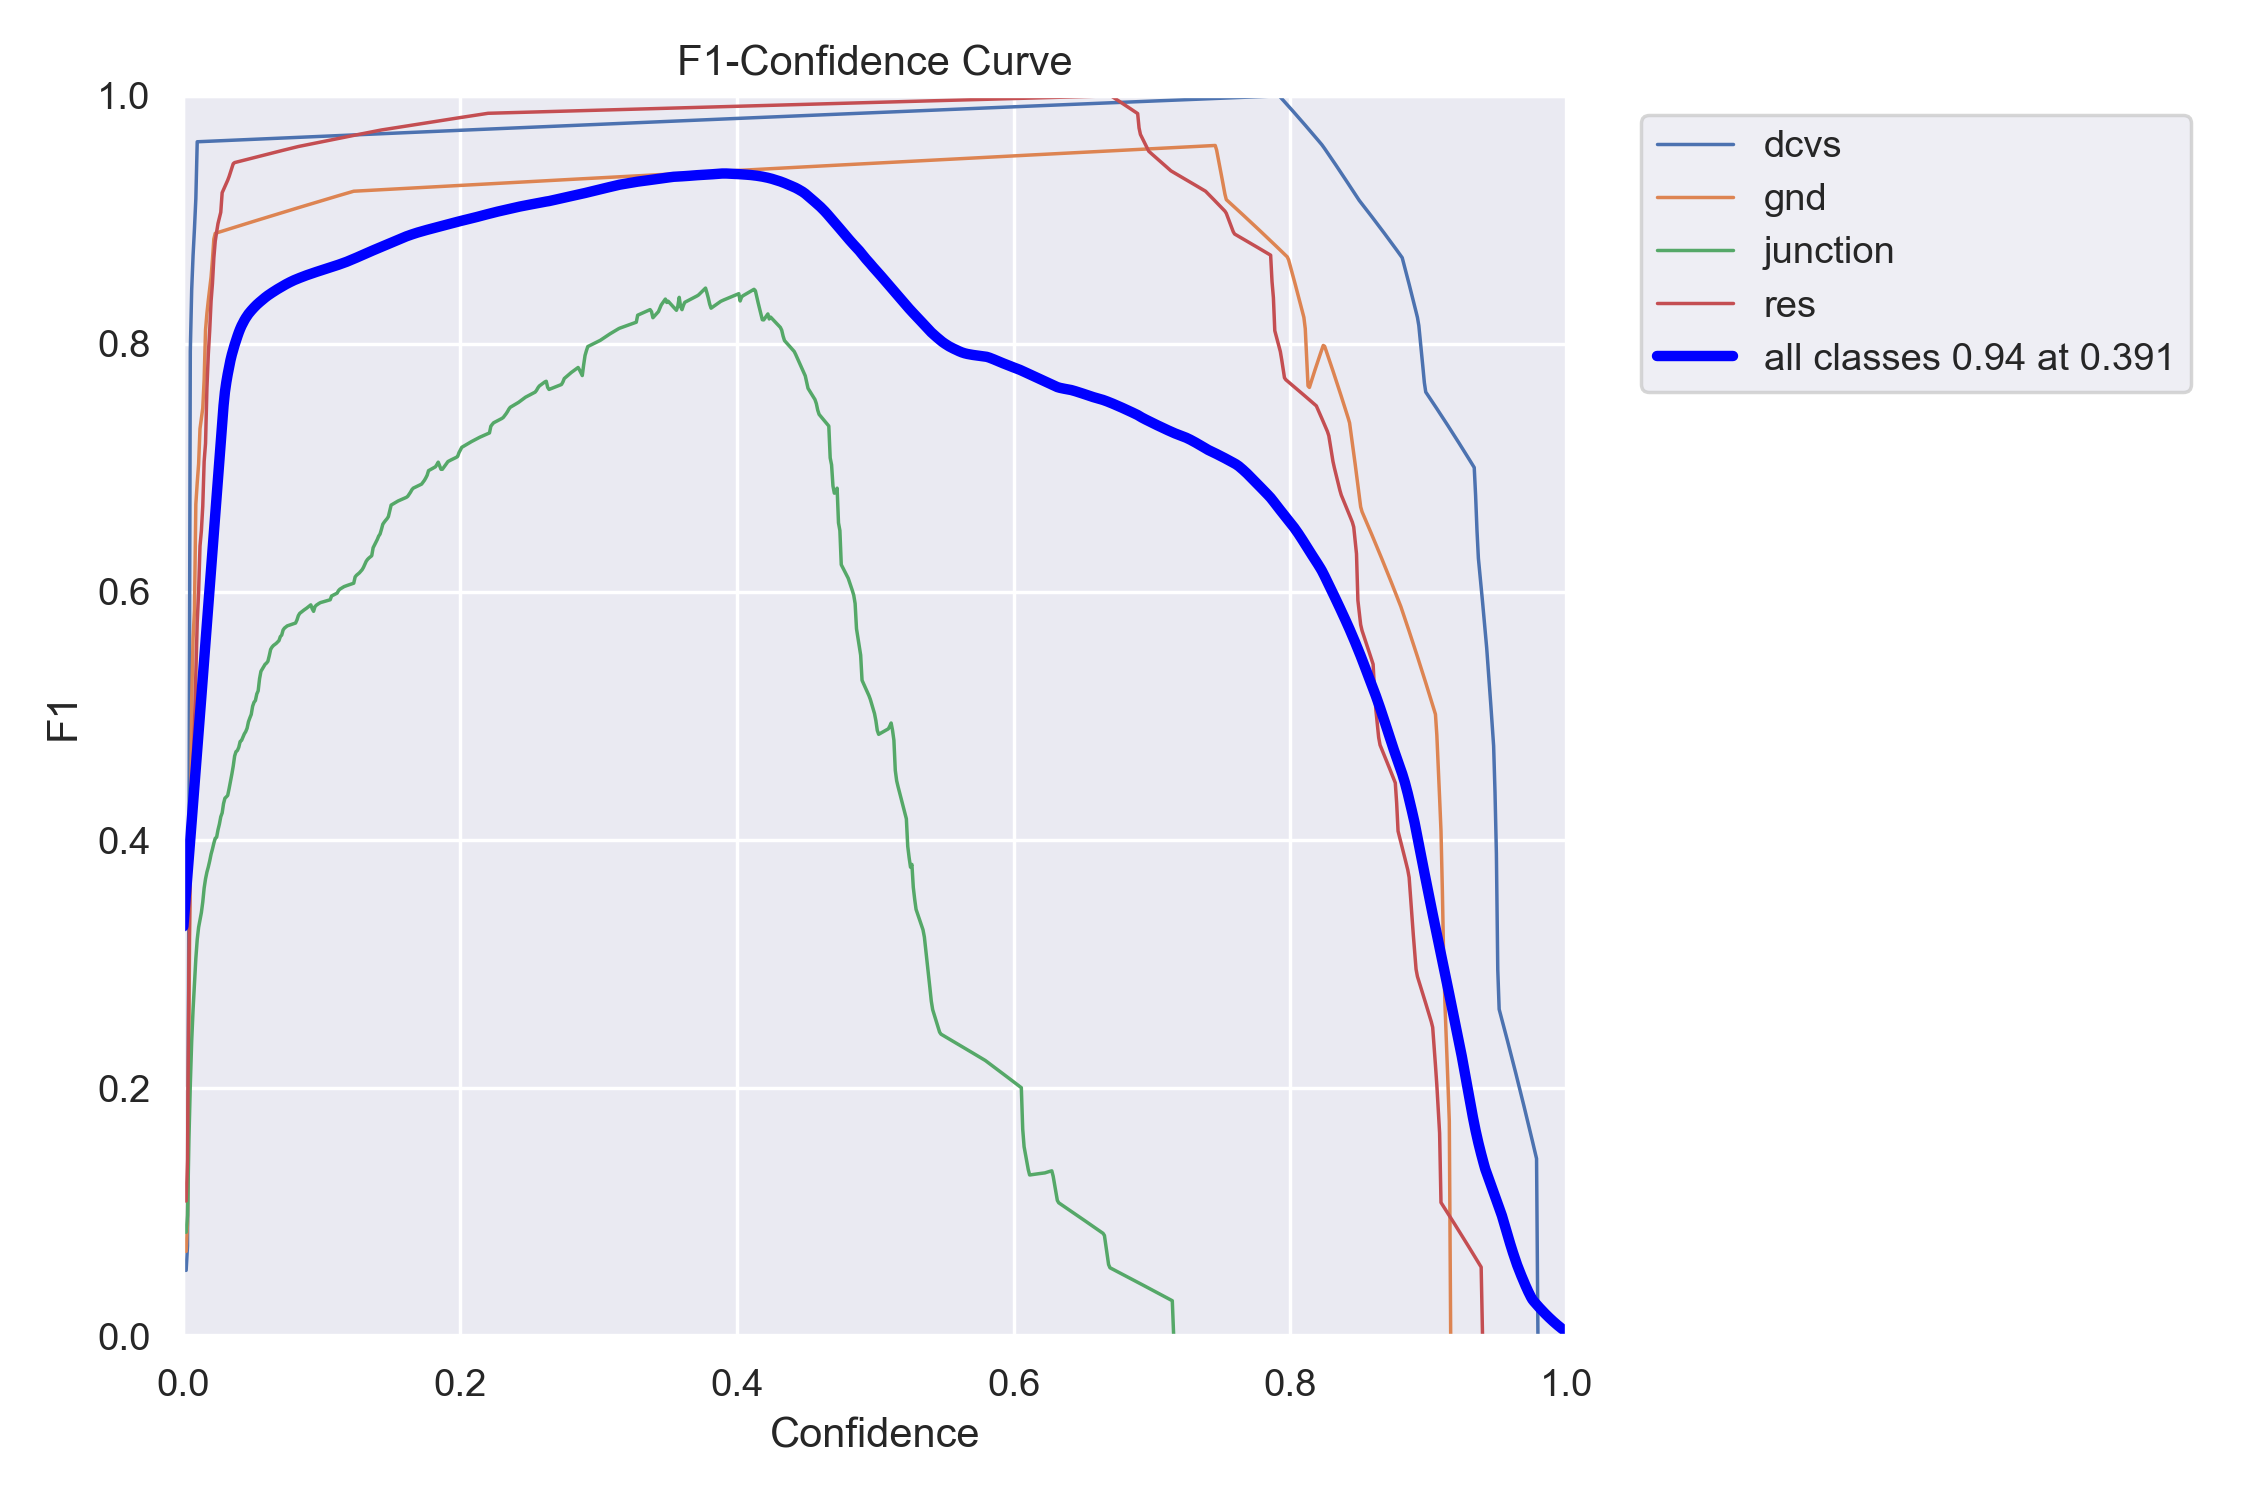
\includegraphics[width=\textwidth]{../common/graphics/poster_F1_curve}
              \caption{F1 Score}
              \label{fig:f1-score for all classes}
            \end{subfigure}
            \begin{subfigure}{0.45\textwidth}
              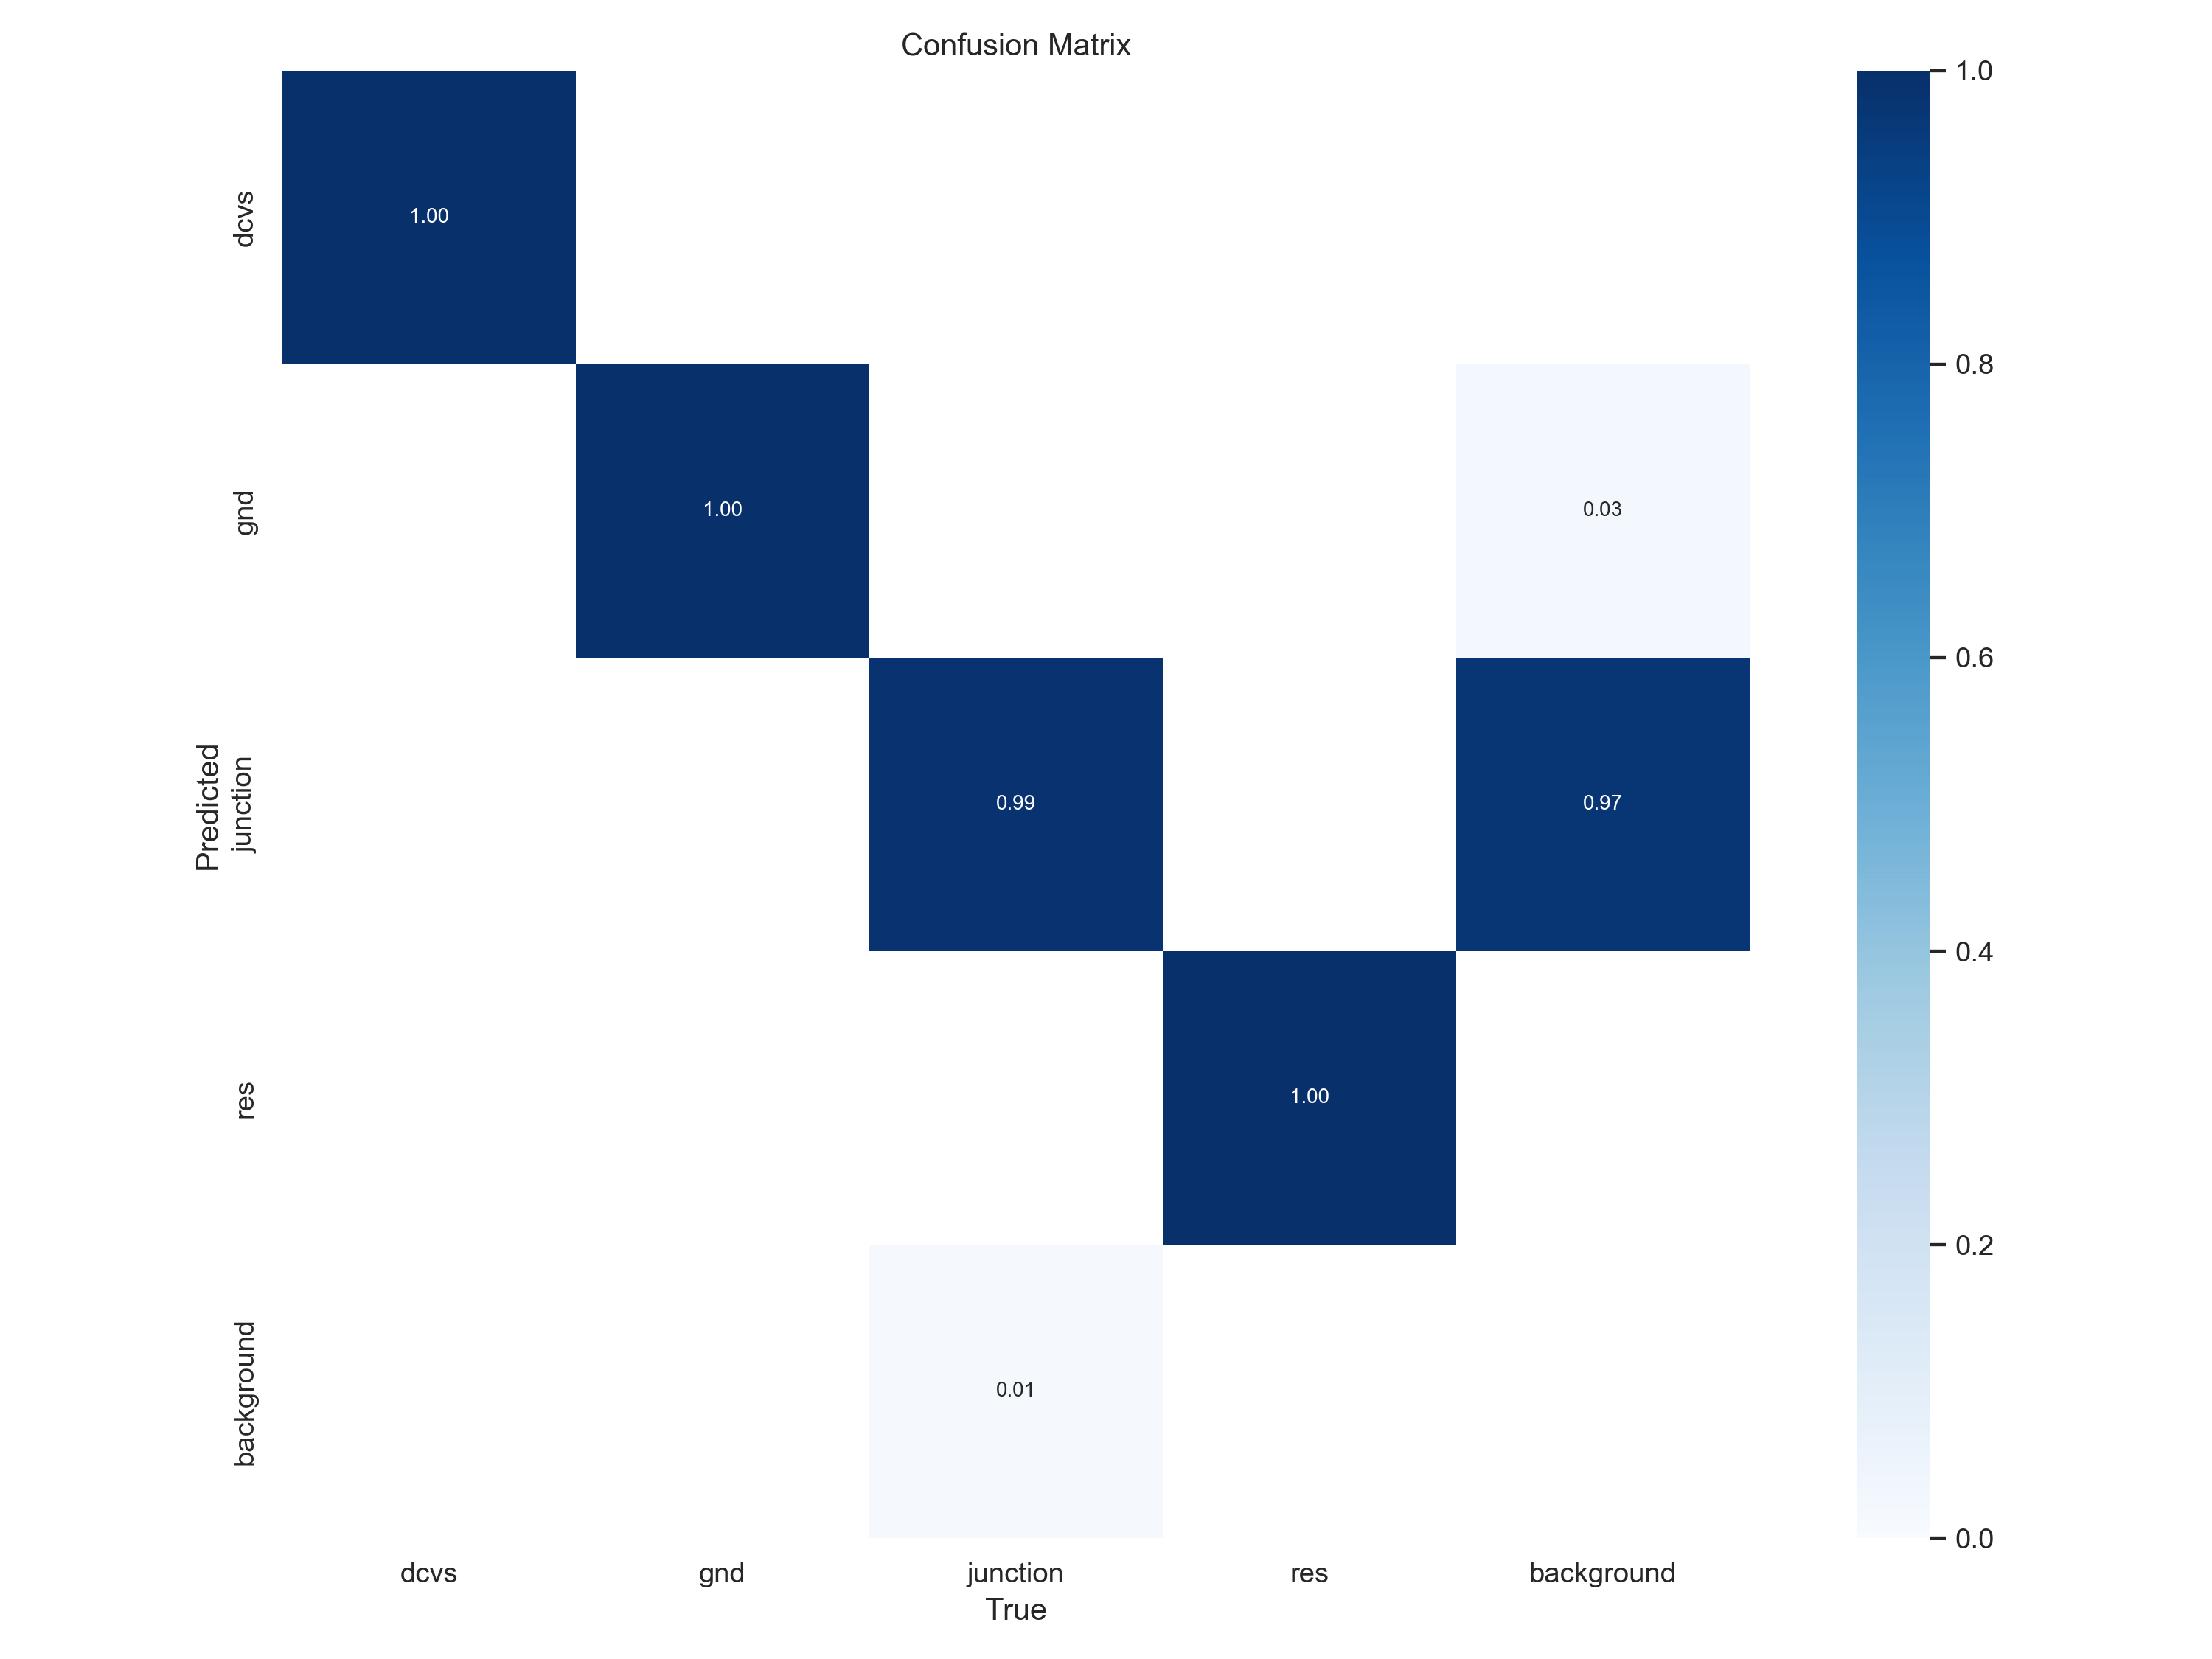
\includegraphics[width=\textwidth]{../common/graphics/poster_confusion_matrix}
              \caption{Confusion Matrix}
              \label{fig:confusion matrix for all classes}
            \end{subfigure}
            \caption{
              \centering
              Component detection accuracy as F1 Score and confusion matrix.
              Demonstration available at QR code at the end of this document.}
            \label{fig:f1-score-confusion-matrix}
          \end{figure}
        \end{block}
      }

      \begin{block}{5. Findings}
        Using deep learning techniques in the form of the latest advancements
        in object detection algorithms, YOLOv8 \cite{}, a high F1-score was
        achieved for all classes except junctions (figure~\ref{fig:f1-score for all classes}, green line).

        A welcome discovery was made where the detector can function directly on CAD images.
        This is a promising result, as it means that the detector can be trained on more
        complex schematics that are CAD generated in the future.

        An improvement that was found is that junction classes can be replaced by node detection
        which is a more reliable means of detecting the intersection of wires.
      \end{block}

      \begin{block}{6. Ongoing and Future Work}
        \begin{itemize}
          \item \textbf{Ongoing Work:}
                \begin{itemize}
                  \normalsize
                  \item[--] Interpret the circuit diagram and produce a simulation file.
                  \item[--] Run the simulation using a Python interface to LT-SPICE.
                  \item[--] Design a user interface for the application to allow the
                    simulation to be displayed on the user's device.
                \end{itemize}
          \item \textbf{Future Work:}
                \normalsize
                \begin{itemize}
                  \normalsize
                  \item[--] Increase the set of detectable components by training the
                    detector on schematics including analogue voltage sources, capacitors,
                    inductors, diodes, transistors, and operational amplifiers.
                \end{itemize}
        \end{itemize}
      \end{block}

      \begin{block}{7. References}
        \nocite{*}
        \footnotesize{
          \bibliographystyle{plain}
          \bibliography{../common/sources}
        }
      \end{block}

    \end{column}

    \separatorcolumn

  \end{columns}

  \end{frame}

\end{document}